\documentclass[
    left=2.5cm,
    right=2.5cm,
    top=2.5cm,
    bottom=3cm,
    bindingoffset=6mm,
    nohyphenation=false
]{szablon/eiti/eiti-thesis}

\langpol
\graphicspath{{rysunki/}}
\addbibresource{bibliografia.bib}

% Dodanie usuwa jedno z ostrzeżeń
\usepackage{csquotes}
% Dodanie tego wpływa na wyświetlanie zdjęć w odpowiedni sposób przy adnotacji [H]
\usepackage{float}
\usepackage{subfig}
\usepackage{amsmath}
\usepackage{amssymb}
\usepackage{booktabs}
\usepackage{multirow}
\usepackage{tikz}
\usetikzlibrary{shapes.geometric, arrows.meta, positioning, fit, calc, backgrounds, decorations.pathreplacing}
\usepackage{pgfplots}
\pgfplotsset{compat=1.18}
\usepackage[ruled,vlined,linesnumbered]{algorithm2e}
\SetAlgorithmName{Algorytm}{Algorytm}{Spis algorytmów}
\usepackage{listings}
\lstset{
    language=Python,
    basicstyle=\ttfamily\small,
    keywordstyle=\bfseries\color{blue!70!black},
    commentstyle=\itshape\color{green!50!black},
    stringstyle=\color{red!60!black},
    numbers=left,
    numberstyle=\tiny\color{gray},
    numbersep=5pt,
    breaklines=true,
    frame=single,
    captionpos=b,
    tabsize=4
}

\begin{document}

\DiplomaThesis
\instytut{TODO: Nazwa instytutu}
\kierunek{TODO: Kierunek studiów}
\specjalnosc{TODO: Specjalność}
\title{
     Framework do predykcji mutacji aminokwasowych w białkach wirusowych z~wykorzystaniem rekurencyjnych sieci neuronowych
}
\engtitle{
    A Framework for Predicting Amino Acid Mutations in Virus Proteins Using Recurrent Neural Networks
}
\author{Filip Korzeniewski}
\album{TODO: Numer albumu}
\promotor{dr hab. inż. Tomasz Gambin}
\date{\the\year}
\maketitle

%--------------------------------------
% Streszczenie po polsku
%--------------------------------------
\cleardoublepage % Zaczynamy od nieparzystej strony
\streszczenie

Mutacje aminokwasowe w~białkach wirusowych stanowią kluczowy czynnik warunkujący zdolność patogenów do unikania odpowiedzi immunologicznej gospodarza. Zdolność do przewidywania przyszłych mutacji w~regionach epitopowych białek powierzchniowych wirusów ma istotne znaczenie dla projektowania szczepionek i~monitorowania epidemiologicznego. Niniejsza praca przedstawia konfigurowalny framework do predykcji mutacji aminokwasowych w~białkach wirusowych z~wykorzystaniem rekurencyjnych sieci neuronowych.

Zaproponowany potok przetwarzania obejmuje następujące etapy: parsowanie sekwencji w~formacie FASTA, kodowanie aminokwasów metodą ProtVec, klasteryzację sekwencji algorytmem K-means w~ramach poszczególnych okresów czasowych, łączenie klastrów między kolejnymi okresami na podstawie odległości centroidów oraz generowanie próbek treningowych z~wykorzystaniem okna przesuwnego. Framework udostępnia trzy architektury modeli predykcyjnych: standardową sieć LSTM, LSTM z~mechanizmem atencji temporalnej (Attention LSTM) oraz LSTM z~podwójnym mechanizmem atencji operującym zarówno w~wymiarze czasowym, jak i~wymiarze cech (Dual Attention LSTM).

Ewaluację przeprowadzono na dwóch zbiorach danych: sekwencjach białka S (Spike) wirusa SARS-CoV-2 pozyskanych z~bazy GISAID oraz sekwencjach białka hemagglutyniny (HA) wirusa Influenza A podtypu H1N1 z~bazy NCBI.
% TODO: Uzupełnić wyniki --- np.: Model Dual Attention LSTM osiągnął najwyższe
% wartości współczynnika korelacji Matthewsa (MCC) wynoszące odpowiednio
% X,XX dla SARS-CoV-2 i Y,YY dla Influenza, przewyższając zarówno model bazowy
% (regresja logistyczna), jak i standardową architekturę LSTM.
Zaprojektowany framework charakteryzuje się konfigurowalnością opartą na plikach YAML, reprodukowalnością eksperymentów oraz rozszerzalnością umożliwiającą zastosowanie do nowych białek wirusowych bez modyfikacji kodu źródłowego.

\slowakluczowe predykcja mutacji, SARS-CoV-2, Influenza, LSTM, mechanizm atencji, ProtVec, klasteryzacja

%--------------------------------------
% Streszczenie po angielski
%--------------------------------------
\newpage % Rozdziały zaczynamy od nowej strony.

\abstract

Summary in English.....

\keywords ChatGPT, Buzzword300



% Oświadczenie o autorstwie
\cleardoublepage  % Zaczynamy od nieparzystej strony
\pagestyle{plain}
\makeauthorship

% Spis treści
\cleardoublepage % Zaczynamy od nieparzystej strony
\tableofcontents

% Rozdziały
\cleardoublepage % Zaczynamy od nieparzystej strony
\pagestyle{headings}
\newpage
\section{Wstęp}

Pandemia wywołana przez wirusa SARS-CoV-2, ogłoszona przez Światową Organizację Zdrowia w~marcu 2020~roku, stanowiła jedno z~najpoważniejszych zagrożeń zdrowia publicznego w~najnowszej historii. Równocześnie sezonowe epidemie grypy, wywoływane między innymi przez wirusy Influenza~A, od dziesięcioleci pozostają istotnym problemem epidemiologicznym, powodując setki tysięcy zgonów rocznie na całym świecie. W~obu przypadkach kluczową rolę w~procesie infekcji odgrywają białka powierzchniowe wirusa --- białko Spike~(S) w~przypadku SARS-CoV-2 oraz hemaglutynina~(HA) w~przypadku wirusa grypy~\cite{walls2020spike, bush1999influenza}. Białka te są głównym celem odpowiedzi immunologicznej gospodarza, a~zarazem stanowią podstawowy antygen wykorzystywany w~konstrukcji szczepionek. Mutacje zachodzące w~regionach epitopowych tych białek prowadzą do zjawiska ucieczki immunologicznej (ang.~\textit{immune escape}), w~wyniku którego wcześniej nabyta odporność --- zarówno poszczepienną, jak i~poinfekcyjna --- może okazać się niewystarczająca wobec nowych wariantów wirusa~\cite{harvey2021variants}. Konsekwencją tego procesu jest konieczność cyklicznej aktualizacji składu szczepionek, co wymaga ciągłego monitorowania ewolucji genomowej patogenów.

Dynamiczny rozwój technologii sekwencjonowania nowej generacji doprowadził do bezprecedensowego wzrostu liczby dostępnych danych sekwencyjnych. Baza GISAID (ang.~\textit{Global Initiative on Sharing All Influenza Data}) zgromadziła ponad 15~milionów sekwencji genomowych wirusa SARS-CoV-2, natomiast baza NCBI Influenza Virus Resource udostępnia wieloletnie dane dotyczące wirusów grypy~\cite{elbe2017gisaid, bao2008ncbi}. Tak ogromna skala danych sprawia, że tradycyjne metody analizy filogenetycznej stają się niewystarczające, co motywuje poszukiwanie podejść opartych na uczeniu maszynowym. W~ostatnich latach zaproponowano szereg metod predykcji ewolucji wirusów, obejmujących zarówno modele językowe białek~\cite{hie2021viral}, jak i~podejścia statystyczne identyfikujące czynniki napędzające pojawianie się nowych wariantów~\cite{maher2022predicting}. Niemniej jednak niewiele istniejących rozwiązań łączy reprezentacje wektorowe sekwencji białkowych (ang.~\textit{embeddings}) z~rekurencyjnymi sieciami neuronowymi wyposażonymi w~mechanizmy atencji, osadzonymi w~kontekście analizy szeregów czasowych.

Zdolność do przewidywania, w~których regionach białka wirusowego zajdą mutacje w~nadchodzących okresach, ma istotne znaczenie praktyczne. Umożliwia ona proaktywne projektowanie szczepionek, skracając czas reakcji na pojawienie się nowych wariantów. Ponadto istnieje zapotrzebowanie na uniwersalne narzędzia, które nie będą ograniczone do pojedynczego patogenu, lecz pozwolą na analizę różnych białek wirusowych przy minimalnych modyfikacjach konfiguracji. Podejście oparte na klasteryzacji sekwencji w~oknach czasowych, w~połączeniu ze śledzeniem ewolucji klastrów między kolejnymi okresami, oferuje naturalny sposób modelowania dynamiki zmian w~populacji wirusowej.

Wkład niniejszej pracy obejmuje pięć głównych elementów. Po pierwsze, zaprojektowano i~zaimplementowano uniwersalny framework do predykcji mutacji aminokwasowych w~białkach wirusowych, konfigurowalny za pomocą plików YAML dla różnych patogenów. Po drugie, opracowano wieloetapowy potok przetwarzania danych, transformujący surowe pliki FASTA w~gotowy zbiór danych treningowych poprzez czyszczenie sekwencji, podział na okresy czasowe, klasteryzację K-means z~wykorzystaniem reprezentacji ProtVec~\cite{asgari2015protvec} oraz dwukierunkowe łączenie klastrów między kolejnymi okresami. Po trzecie, zaimplementowano i~porównano trzy architektury modeli opartych na rekurencyjnych sieciach neuronowych: bazowy model LSTM~\cite{hochreiter1997lstm}, model LSTM z~mechanizmem atencji Bahdanau~\cite{bahdanau2015attention} oraz model LSTM z~podwójną atencją (ang.~\textit{Dual-Stage Attention-Based RNN}, DA-RNN)~\cite{qin2017darnn}. Po czwarte, przeprowadzono ewaluację eksperymentalną na dwóch zbiorach danych --- sekwencjach białka~S wirusa SARS-CoV-2 oraz białka HA wirusa Influenza~A podtypu H1N1 --- stosując chronologiczny podział danych oraz współczynnik korelacji Matthewsa (ang.~\textit{Matthews Correlation Coefficient}, MCC) jako główną metrykę oceny~\cite{chicco2020mcc}. Po piąte, zapewniono reprodukowalność eksperymentów poprzez konteneryzację środowiska z~wykorzystaniem platformy Docker.

Niniejsza praca składa się z~sześciu rozdziałów. Rozdział~2 formułuje cel pracy, tezę badawczą oraz precyzuje zakres przeprowadzonych badań. Rozdział~3 zawiera przegląd literatury obejmujący podstawy biologiczne, metody reprezentacji sekwencji białkowych, algorytmy klasteryzacji oraz architektury rekurencyjnych sieci neuronowych z~mechanizmami atencji. W~rozdziale~4 przedstawiono szczegółowy opis zaproponowanego rozwiązania, obejmujący architekturę frameworka, potok przetwarzania danych oraz implementację modeli. Rozdział~5 prezentuje wyniki ewaluacji eksperymentalnej na obu zbiorach danych wraz z~analizą porównawczą zastosowanych architektur. Rozdział~6 zawiera podsumowanie pracy, krytyczną analizę osiągniętych rezultatów oraz propozycje kierunków dalszych badań.

\newpage % Rozdziały zaczynamy od nowej strony.
\section{Cel pracy}

Celem niniejszej pracy jest ....... (teza badawcza)


\newpage % Rozdziały zaczynamy od nowej strony.
\section{Przegląd literaratury}

Przegląd literatury związanej z rozwiązywanym problemem. 

W pracy~\cite{he2016deep} opisano ....
W~\cite{liu2022convnet} zaproponowano nowatorską architekturę....
Przykładowy rysunek~\ref{fig:convnext}.

\begin{figure}[h]
    \centering
    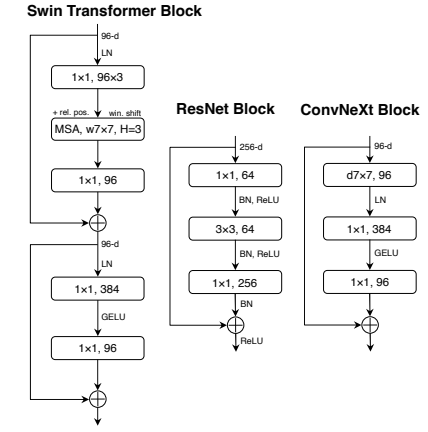
\includegraphics[width=0.5\textwidth]{rysunki/convnext_block.png}
    \caption{Porównanie bloków rezydualnych wykorzystywanych w sieci Swin Transformer, ResNet i ConvNeXt.}
    \label{fig:convnext}
\end{figure}

\newpage
\section{Opis rozwiązania}
\label{sec:opis-rozwiazania}

W niniejszym rozdziale przedstawiono szczegółowy opis frameworka opracowanego na potrzeby predykcji mutacji aminokwasowych w białkach wirusowych. Framework zaimplementowano w języku Python z wykorzystaniem bibliotek PyTorch~\cite{paszke2019pytorch} oraz scikit-learn~\cite{pedregosa2011sklearn}. Całość zaprojektowano jako konfigurowalny potok przetwarzania danych (ang.~\emph{pipeline}), który można dostosować do różnych białek wirusowych poprzez zmianę plików konfiguracyjnych YAML, bez konieczności modyfikacji kodu źródłowego. W dalszej części rozdziału kolejno omówiono architekturę frameworka, poszczególne etapy potoku przetwarzania danych oraz zastosowane architektury sieci neuronowych.

% ============================================================================
\subsection{Architektura frameworka}
\label{subsec:architektura}

Opracowany framework realizuje pełny potok przetwarzania danych -- od surowych sekwencji aminokwasowych w formacie FASTA, przez klasteryzację i tworzenie zbioru danych treningowych, aż po trenowanie i ewaluację modeli rekurencyjnych sieci neuronowych. Potok składa się z pięciu głównych etapów, przedstawionych na rysunku~\ref{fig:pipeline-overview}.

\begin{figure}[H]
\centering
\begin{tikzpicture}[
    block/.style={rectangle, draw=blue!60, fill=blue!8, text width=3.2cm,
                  minimum height=1.6cm, align=center, rounded corners=3pt,
                  font=\small\bfseries},
    arrow/.style={-{Stealth[length=3mm]}, thick, blue!60},
    label/.style={font=\scriptsize, text width=3.2cm, align=center}
]
    \node[block] (prep) {Przygotowanie\\danych};
    \node[block, right=0.8cm of prep] (cluster) {Klasteryzacja};
    \node[block, right=0.8cm of cluster] (link) {Łączenie\\klastrów};
    \node[block, right=0.8cm of link] (dataset) {Tworzenie\\zbioru danych};
    \node[block, right=0.8cm of dataset] (train) {Trenowanie\\modelu};

    \draw[arrow] (prep) -- (cluster);
    \draw[arrow] (cluster) -- (link);
    \draw[arrow] (link) -- (dataset);
    \draw[arrow] (dataset) -- (train);

    \node[label, below=0.3cm of prep] {FASTA $\rightarrow$ CSV\\Filtrowanie\\Podział na okresy};
    \node[label, below=0.3cm of cluster] {ProtVec\\K-means\\Dobór $k$};
    \node[label, below=0.3cm of link] {Odległość\\euklidesowa\\Dwukierunkowe};
    \node[label, below=0.3cm of dataset] {Okno przesuwne\\Epitopy\\Etykiety mutacji};
    \node[label, below=0.3cm of train] {LSTM\\Atencja\\Ewaluacja};
\end{tikzpicture}
\caption{Schemat ogólny potoku przetwarzania danych w opracowanym frameworku. Każdy blok odpowiada jednemu etapowi, który można uruchomić niezależnie.}
\label{fig:pipeline-overview}
\end{figure}

Głównym punktem wejścia frameworka jest skrypt \texttt{main.py}, który udostępnia interfejs wiersza poleceń (ang.~\emph{Command Line Interface}, CLI) z następującymi komendami:

\begin{itemize}
    \item \texttt{prepare} -- przygotowanie danych z plików FASTA,
    \item \texttt{cluster} -- klasteryzacja sekwencji i łączenie klastrów między okresami,
    \item \texttt{dataset} -- tworzenie końcowego zbioru danych treningowych,
    \item \texttt{train} -- trenowanie i ewaluacja modeli,
    \item \texttt{full-pipeline} -- sekwencyjne wykonanie wszystkich etapów.
\end{itemize}

Wszystkie parametry konfiguracyjne -- od formatu danych wejściowych, przez hiperparametry klasteryzacji, aż po architekturę i parametry trenowania modelu -- są zdefiniowane w plikach YAML. Takie podejście umożliwia łatwe dostosowanie frameworka do różnych białek wirusowych. W tabeli~\ref{tab:config-comparison} zestawiono kluczowe różnice konfiguracyjne pomiędzy dwoma badanymi wirusami.

\begin{table}[H]
\centering
\caption{Porównanie konfiguracji frameworka dla białka S wirusa SARS-CoV-2 oraz białka HA wirusa Influenza~A~H1N1.}
\label{tab:config-comparison}
\small
\begin{tabular}{lcc}
\toprule
\textbf{Parametr} & \textbf{SARS-CoV-2 (S)} & \textbf{Influenza A H1N1 (HA)} \\
\midrule
Źródło danych & GISAID~\cite{elbe2017gisaid} & NCBI~\cite{bao2008ncbi} \\
Parsowanie nagłówków & Delimiter (\texttt{|}) & Wyrażenie regularne \\
Długość białka [aa] & 1273 $\pm$ 13 & 565 $\pm$ 20 \\
Podział czasowy & Miesiące & Lata \\
Wymagany kodon stop & Tak & Nie \\
Próg niejednoznaczności & 0\% & 5\% \\
Liczba regionów epitopowych & 16 & 5 \\
Pokrycie epitopowe & 24{,}9\% (317/1273) & 16{,}8\% (95/565) \\
Próg podobieństwa epitopów & 50\% & 80\% \\
Docelowy rozmiar zbioru & 12\,680 & 40\,000 \\
\bottomrule
\end{tabular}
\end{table}

% ============================================================================
\subsection{Etap 1: Przygotowanie danych}
\label{subsec:przygotowanie-danych}

Pierwszy etap potoku odpowiada za transformację surowych danych sekwencyjnych w formacie FASTA do ustrukturyzowanego formatu CSV z podziałem na okresy czasowe. Proces ten obejmuje parsowanie nagłówków, walidację i filtrowanie sekwencji oraz organizację danych w strukturze temporalnej.

\subsubsection{Przetwarzanie plików FASTA}
\label{subsubsec:fasta}

Format FASTA stanowi standardowy format zapisu sekwencji biologicznych, w którym każdy rekord składa się z linii nagłówkowej rozpoczynającej się znakiem \texttt{>} oraz jednej lub więcej linii zawierających sekwencję aminokwasową. Poniżej przedstawiono przykładowy rekord:

\begin{lstlisting}[caption={Przyklad rekordu w formacie FASTA dla bialka S wirusa SARS-CoV-2.}, label={lst:fasta-example}, language={}]
>Spike|hCoV-19/Wuhan/WIV04/2019|2019-12-30|EPI_ISL_402124
MFVFLVLLPLVSSQCVNLTTRTQLPPAY...
\end{lstlisting}

Framework obsługuje dwa tryby parsowania nagłówków FASTA, co umożliwia pracę z różnymi źródłami danych:

\begin{enumerate}
    \item \textbf{Tryb oparty na separatorze} (ang.~\emph{delimiter-based}) -- stosowany dla danych z bazy GISAID~\cite{elbe2017gisaid}. Nagłówek jest dzielony względem skonfigurowanego separatora (np.~\texttt{|}), a pozycje poszczególnych pól (gen, izolat, znacznik czasu, numer akcesji) są odczytywane z konfiguracji.
    \item \textbf{Tryb oparty na wyrażeniach regularnych} (ang.~\emph{regex-based}) -- stosowany dla danych z bazy NCBI~\cite{bao2008ncbi}, gdzie struktura nagłówków jest mniej regularna. Używa grup nazwanych w wyrażeniu regularnym do ekstrakcji pól.
\end{enumerate}

W obu trybach wyodrębniane są następujące informacje: nazwa izolatu (\texttt{isolate\_name}), znacznik czasu (\texttt{timestamp}), sekwencja aminokwasowa (\texttt{sequence}) oraz nazwa genu (\texttt{gene}). Znaczniki czasu są normalizowane do formatu \texttt{YYYY-MM-DD}, z możliwością konfiguracji domyślnych wartości dla brakujących komponentów (np.~domyślny miesiąc \texttt{07} dla danych rocznych Influenzy).

\subsubsection{Czyszczenie sekwencji}
\label{subsubsec:czyszczenie}

Etap czyszczenia realizuje wieloetapową filtrację sekwencji, której celem jest usunięcie danych niskiej jakości, które mogłyby negatywnie wpłynąć na dalsze etapy potoku:

\begin{enumerate}
    \item \textbf{Walidacja kodonu stop} -- dla białka S wirusa SARS-CoV-2 wymagane jest, aby sekwencja kończyła się znakiem gwiazdki (\texttt{*}), oznaczającym kodon stop. Dla białka HA Influenzy walidacja ta jest wyłączona, ponieważ bazy danych często nie uwzględniają tego znaku.

    \item \textbf{Filtrowanie aminokwasów niejednoznacznych} -- usuwane są sekwencje zawierające znaki reprezentujące aminokwasy niejednoznaczne: \texttt{X} (nieznany), \texttt{B} (asparagina lub kwas asparaginowy), \texttt{Z} (glutamina lub kwas glutaminowy), \texttt{J} (leucyna lub izoleucyna) oraz \texttt{-} (przerwa w dopasowaniu). Próg tolerancji jest konfigurowalny: 0\% dla SARS-CoV-2 (żadne niejednoznaczne aminokwasy nie są dopuszczalne) oraz 5\% dla Influenzy (dopuszczalny niewielki udział niejednoznacznych reszt).

    \item \textbf{Filtrowanie po długości} -- sekwencje, których długość odbiega od oczekiwanej wartości o więcej niż skonfigurowany margines błędu, są odrzucane. Dla białka S wirusa SARS-CoV-2 oczekiwana długość wynosi 1273~aminokwasów z marginesem $\pm 13$, natomiast dla białka HA Influenzy -- 565~aminokwasów z marginesem $\pm 20$.
\end{enumerate}

Dla dużych plików (powyżej 10~MB) zastosowano przetwarzanie strumieniowe (ang.~\emph{streaming}), które operuje na fragmentach danych (ang.~\emph{chunks}), co ogranicza zużycie pamięci operacyjnej.

\subsubsection{Podział na okresy czasowe}
\label{subsubsec:okresy}

Po oczyszczeniu sekwencje są sortowane według znaczników czasu i grupowane w okresy czasowe. Framework wspiera trzy strategie podziału:

\begin{itemize}
    \item \textbf{Miesięczna} -- stosowana dla SARS-CoV-2, gdzie dane obejmują okres od lutego 2020 do stycznia 2022 (24 okresy),
    \item \textbf{Kwartalna} -- opcja pośrednia, dostępna dla zbiorców o umiarkowanej granularności,
    \item \textbf{Roczna} -- stosowana dla Influenzy, gdzie dane obejmują kilkadziesiąt lat obserwacji.
\end{itemize}

W obrębie każdego okresu usuwane są duplikaty na podstawie nazwy izolatu, a następnie tworzone są pliki z unikalnymi sekwencjami (deduplikacja na podstawie treści sekwencji). Podział na okresy jest kluczowy dla dalszych etapów, ponieważ umożliwia śledzenie ewolucji wirusa w czasie.

% ============================================================================
\subsection{Etap 2: Transformacja ProtVec i klasteryzacja}
\label{subsec:klasteryzacja}

Drugi etap potoku obejmuje transformację sekwencji aminokwasowych do reprezentacji wektorowych oraz ich grupowanie za pomocą algorytmu K-means.

\subsubsection{Transformacja sekwencji do wektorów ProtVec}
\label{subsubsec:protvec}

Do uzyskania numerycznej reprezentacji sekwencji aminokwasowych zastosowano metodę ProtVec, zaproponowaną przez Asgari i Mofrada~\cite{asgari2015protvec}. Metoda ta stanowi adaptację techniki Word2Vec~\cite{mikolov2013word2vec} -- oryginalnie opracowanej do przetwarzania języka naturalnego -- do dziedziny sekwencji biologicznych. Analogia polega na traktowaniu sekwencji białka jak ``zdania'', a krótkich fragmentów aminokwasowych jak ``słów''.

Transformacja sekwencji do wektora ProtVec przebiega w trzech krokach, zilustrowanych na rysunku~\ref{fig:protvec-transform}:

\begin{enumerate}
    \item \textbf{Tworzenie nakładających się trigramów} -- sekwencja aminokwasowa jest dzielona na nakładające się fragmenty o długości 3 aminokwasów (tzw.~3-gramy lub trigramy). Na przykład sekwencja \texttt{MFVFLV} generuje następujące trigramy: [\texttt{MFV}, \texttt{FVF}, \texttt{VFL}, \texttt{FLV}]. Ogólnie, sekwencja o długości $n$ generuje $n - 2$ trigramów.

    \item \textbf{Mapowanie trigramów na wektory} -- każdy trigram jest mapowany na wektor 100-wymiarowy z pretrenowanej macierzy zanurzeń (ang.~\emph{embeddings}). Macierz ta zawiera reprezentacje wektorowe dla 9048 unikalnych trigramów aminokwasowych i została wytrenowana metodą Skip-gram na zbiorze 546\,790 sekwencji z bazy Swiss-Prot~\cite{asgari2015protvec}.

    \item \textbf{Sumowanie wektorów} -- wektory wszystkich trigramów danej sekwencji są sumowane elementowo, co daje jeden wektor 100-wymiarowy reprezentujący całą sekwencję:
\end{enumerate}

\begin{equation}
\label{eq:protvec}
\mathbf{v}_{\text{seq}} = \sum_{i=1}^{n-2} \mathbf{e}(t_i)
\end{equation}

\noindent gdzie $\mathbf{e}(t_i) \in \mathbb{R}^{100}$ oznacza wektor zanurzenia trigramu $t_i$, a $n$ jest długością sekwencji aminokwasowej.

\begin{figure}[H]
\centering
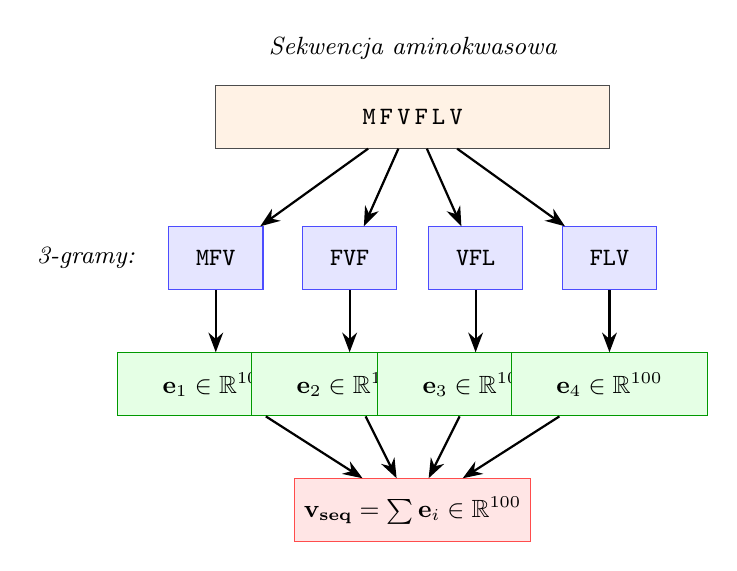
\begin{tikzpicture}[
    seqbox/.style={rectangle, draw=black!70, fill=orange!10, minimum height=0.8cm,
                   minimum width=1cm, font=\ttfamily\small},
    tribox/.style={rectangle, draw=blue!70, fill=blue!10, minimum height=0.8cm,
                   minimum width=1.2cm, font=\ttfamily\small},
    vecbox/.style={rectangle, draw=green!60!black, fill=green!10, minimum height=0.8cm,
                   minimum width=2.5cm, font=\small},
    sumbox/.style={rectangle, draw=red!70, fill=red!10, minimum height=0.8cm,
                   minimum width=3cm, font=\small\bfseries},
    arrow/.style={-{Stealth[length=2.5mm]}, thick},
    label/.style={font=\small\itshape}
]
    % Sequence
    \node[seqbox, minimum width=5cm] (seq) at (0, 0) {M\,F\,V\,F\,L\,V};
    \node[label, above=0.2cm of seq] {Sekwencja aminokwasowa};

    % Trigrams
    \node[tribox] (t1) at (-2.5, -1.8) {MFV};
    \node[tribox] (t2) at (-0.8, -1.8) {FVF};
    \node[tribox] (t3) at (0.8, -1.8) {VFL};
    \node[tribox] (t4) at (2.5, -1.8) {FLV};
    \node[label, left=0.3cm of t1] {3-gramy:};

    \draw[arrow] (seq) -- (t1);
    \draw[arrow] (seq) -- (t2);
    \draw[arrow] (seq) -- (t3);
    \draw[arrow] (seq) -- (t4);

    % Vectors
    \node[vecbox] (v1) at (-2.5, -3.4) {$\mathbf{e}_1 \in \mathbb{R}^{100}$};
    \node[vecbox] (v2) at (-0.8, -3.4) {$\mathbf{e}_2 \in \mathbb{R}^{100}$};
    \node[vecbox] (v3) at (0.8, -3.4) {$\mathbf{e}_3 \in \mathbb{R}^{100}$};
    \node[vecbox] (v4) at (2.5, -3.4) {$\mathbf{e}_4 \in \mathbb{R}^{100}$};

    \draw[arrow] (t1) -- (v1);
    \draw[arrow] (t2) -- (v2);
    \draw[arrow] (t3) -- (v3);
    \draw[arrow] (t4) -- (v4);

    % Sum
    \node[sumbox] (sum) at (0, -5.0) {$\mathbf{v}_{\text{seq}} = \sum \mathbf{e}_i \in \mathbb{R}^{100}$};

    \draw[arrow] (v1) -- (sum);
    \draw[arrow] (v2) -- (sum);
    \draw[arrow] (v3) -- (sum);
    \draw[arrow] (v4) -- (sum);
\end{tikzpicture}
\caption{Schemat transformacji sekwencji aminokwasowej do wektora ProtVec. Sekwencja jest dzielona na nakładające się trigramy, każdy trigram jest mapowany na wektor 100-wymiarowy, a następnie wektory są sumowane.}
\label{fig:protvec-transform}
\end{figure}

Dla optymalizacji wydajności zaimplementowano procesor wsadowy (\texttt{BatchVectorProcessor}), który wykorzystuje słownik trigramów z pamięcią podręczną (ang.~\emph{LRU cache}) oraz prealokowane tablice NumPy, co pozwala uniknąć kosztownych alokacji pamięci przy przetwarzaniu dużych zbiorów danych.

\subsubsection{Klasteryzacja K-means z automatycznym doborem $k$}
\label{subsubsec:kmeans}

Po transformacji sekwencji do przestrzeni ProtVec, wektory w obrębie każdego okresu czasowego są grupowane za pomocą algorytmu K-means~\cite{macqueen1967kmeans}. Klasteryzacja służy redukcji redundancji danych -- zamiast przechowywać informacje o każdej sekwencji, dalsza analiza operuje na centroidach klastrów, które reprezentują typowe warianty wirusa w danym okresie.

Framework implementuje automatyczny dobór optymalnej liczby klastrów $k$ z wykorzystaniem współczynnika sylwetkowego (ang.~\emph{Silhouette Score})~\cite{rousseeuw1987silhouette}. Dla każdego okresu czasowego testowane są wartości $k$ z zakresu $[k_{\min}, k_{\max}]$ (domyślnie $[2, 19]$), a wybierana jest wartość maksymalizująca współczynnik sylwetkowy:

\begin{equation}
\label{eq:silhouette-impl}
k^{*} = \arg\max_{k \in [k_{\min}, k_{\max}]} S(k)
\end{equation}

\noindent gdzie $S(k)$ oznacza średni współczynnik sylwetkowy dla podziału na $k$ klastrów. Współczynnik sylwetkowy mierzy, jak dobrze każda próbka jest przypisana do swojego klastra w porównaniu do najbliższego sąsiedniego klastra, przyjmując wartości z przedziału $[-1, 1]$.

W zależności od liczby próbek w danym okresie, framework automatycznie wybiera wariant algorytmu:

\begin{itemize}
    \item \textbf{Standardowy K-means} -- dla okresów z $\leq 2000$ próbkami, z parametrami: \texttt{n\_init}$=10$ (liczba losowych inicjalizacji), \texttt{max\_iter}$=300$ (maksymalna liczba iteracji).
    \item \textbf{Mini-Batch K-means}~\cite{sculley2010minibatch} -- dla okresów z $> 2000$ próbkami, z parametrami: \texttt{batch\_size}$=500$, \texttt{n\_init}$=3$. Wariant ten przetwarza losowe podpróbki danych w każdej iteracji, co znacząco przyspiesza obliczenia kosztem niewielkiej utraty dokładności.
\end{itemize}

Wynikiem klasteryzacji każdego okresu są: etykiety klastrów przypisane do poszczególnych sekwencji oraz centroidy -- 100-wymiarowe wektory w przestrzeni ProtVec reprezentujące środki klastrów.

% ============================================================================
\subsection{Etap 3: Łączenie klastrów między okresami}
\label{subsec:laczenie-klastrow}

Po klasteryzacji sekwencji w poszczególnych okresach czasowych konieczne jest ustanowienie powiązań między klastrami z kolejnych okresów. Powiązania te umożliwiają śledzenie ewolucji wariantów wirusa w czasie i stanowią podstawę do tworzenia łańcuchów sekwencji w kolejnym etapie.

Zastosowano dwukierunkowy algorytm łączenia centroidów oparty na odległości euklidesowej w 100-wymiarowej przestrzeni ProtVec. Algorytm składa się z trzech kroków, zilustrowanych na rysunku~\ref{fig:cluster-linking}:

\begin{enumerate}
    \item \textbf{Łączenie w przód} (ang.~\emph{forward linking}) -- dla każdego centroidu w okresie $t$ wyznaczany jest najbliższy centroid w okresie $t+1$ na podstawie odległości euklidesowej:
    \begin{equation}
    \label{eq:forward-link}
    f(c_i^{(t)}) = \arg\min_{c_j^{(t+1)}} \left\| c_i^{(t)} - c_j^{(t+1)} \right\|_2
    \end{equation}

    \item \textbf{Łączenie wstecz} (ang.~\emph{backward linking}) -- analogicznie, dla każdego centroidu w okresie $t+1$ wyznaczany jest najbliższy centroid w okresie $t$:
    \begin{equation}
    \label{eq:backward-link}
    b(c_j^{(t+1)}) = \arg\min_{c_i^{(t)}} \left\| c_j^{(t+1)} - c_i^{(t)} \right\|_2
    \end{equation}

    \item \textbf{Scalanie wyników} -- powiązania uzyskane w obu kierunkach są łączone w zbiór unikalnych par, a duplikaty są usuwane. Wynikowe powiązania są zapisywane w kolumnie \texttt{next\_cluster}, gdzie identyfikatory powiązanych klastrów są oddzielone myślnikiem (np.~\texttt{0-1-2} oznacza powiązanie z klastrami 0, 1 i 2 w następnym okresie).
\end{enumerate}

\begin{figure}[H]
\centering
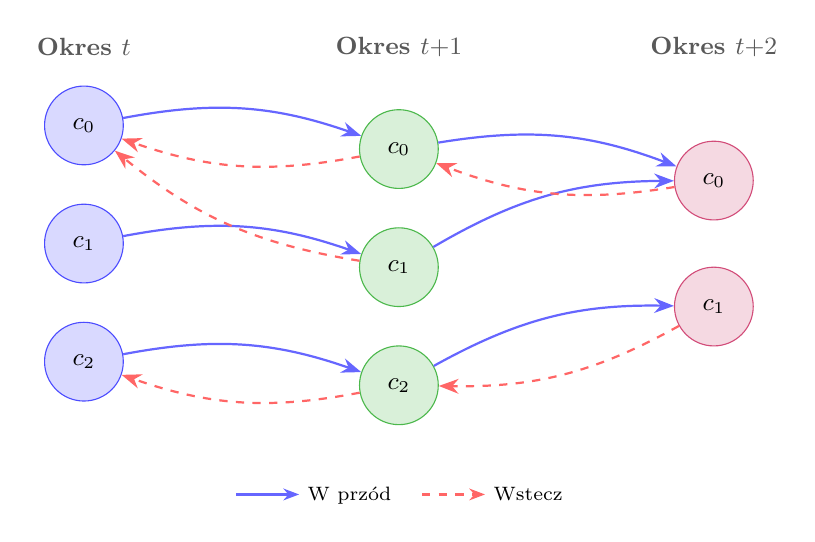
\begin{tikzpicture}[
    cluster/.style={circle, draw=#1!70, fill=#1!15, minimum size=1cm,
                    font=\small\bfseries, inner sep=0pt},
    period/.style={font=\small\bfseries, text=gray!70!black},
    fwd/.style={-{Stealth[length=2.5mm]}, thick, blue!60, bend left=15},
    bwd/.style={-{Stealth[length=2.5mm]}, thick, red!60, bend left=15, dashed}
]
    % Period labels
    \node[period] at (0, 2.5) {Okres $t$};
    \node[period] at (4, 2.5) {Okres $t{+}1$};
    \node[period] at (8, 2.5) {Okres $t{+}2$};

    % Period t clusters
    \node[cluster=blue] (a0) at (0, 1.5) {$c_0$};
    \node[cluster=blue] (a1) at (0, 0) {$c_1$};
    \node[cluster=blue] (a2) at (0, -1.5) {$c_2$};

    % Period t+1 clusters
    \node[cluster=green!60!black] (b0) at (4, 1.2) {$c_0$};
    \node[cluster=green!60!black] (b1) at (4, -0.3) {$c_1$};
    \node[cluster=green!60!black] (b2) at (4, -1.8) {$c_2$};

    % Period t+2 clusters
    \node[cluster=purple] (c0) at (8, 0.8) {$c_0$};
    \node[cluster=purple] (c1) at (8, -0.8) {$c_1$};

    % Forward links (blue, solid)
    \draw[fwd] (a0) to (b0);
    \draw[fwd] (a1) to (b1);
    \draw[fwd] (a2) to (b2);

    % Backward links (red, dashed)
    \draw[bwd] (b0) to (a0);
    \draw[bwd] (b1) to (a0);
    \draw[bwd] (b2) to (a2);

    % Forward links period t+1 -> t+2
    \draw[fwd] (b0) to (c0);
    \draw[fwd] (b1) to (c0);
    \draw[fwd] (b2) to (c1);

    % Backward links period t+2 -> t+1
    \draw[bwd] (c0) to (b0);
    \draw[bwd] (c1) to (b2);

    % Legend
    \node[font=\scriptsize] at (4, -3.2) {
        \tikz{\draw[-{Stealth[length=2mm]}, thick, blue!60] (0,0) -- (0.8,0);} W przód \quad
        \tikz{\draw[-{Stealth[length=2mm]}, thick, red!60, dashed] (0,0) -- (0.8,0);} Wstecz
    };
\end{tikzpicture}
\caption{Dwukierunkowy algorytm łączenia klastrów między trzema kolejnymi okresami czasowymi. Strzałki ciągłe (niebieskie) oznaczają łączenie w przód, strzałki przerywane (czerwone) -- łączenie wstecz.}
\label{fig:cluster-linking}
\end{figure}

Podejście dwukierunkowe zapewnia pełniejsze odwzorowanie ewolucyjnych zależności między wariantami -- uwzględnia zarówno sytuacje, w których jeden wariant ewoluuje w wiele potomnych (dywergencja), jak i przypadki, gdy wiele wariantów zbiega do jednego (konwergencja).

% ============================================================================
\subsection{Etap 4: Tworzenie zbioru danych}
\label{subsec:tworzenie-zbioru}

Czwarty etap stanowi najbardziej złożone ogniwo potoku, w którym powiązane klastry są transformowane w końcowy zbiór danych treningowych z etykietami mutacji.

\subsubsection{Mechanizm okna przesuwnego}
\label{subsubsec:okno-przesuwne}

Do tworzenia próbek treningowych zastosowano mechanizm okna przesuwnego (ang.~\emph{sliding window}) o konfigurowalnym rozmiarze $w$ (domyślnie $w = 10$ kolejnych okresów czasowych). W obrębie każdego okna:

\begin{itemize}
    \item \textbf{Wejście} ($\mathbf{x}$): sekwencje z okresów $t_1, t_2, \ldots, t_{w-1}$ stanowią ciąg wejściowy modelu,
    \item \textbf{Cel} ($y$): sekwencja z okresu $t_w$ stanowi cel predykcji (etykietę mutacji).
\end{itemize}

Okno jest przesuwane o jeden okres, co generuje kolejne próbki treningowe. Na przykład dla 24 okresów miesięcznych i okna $w = 10$, uzyskuje się 15 możliwych pozycji okna.

\begin{figure}[H]
\centering
\begin{tikzpicture}[
    period/.style={rectangle, draw=gray!60, fill=gray!10, minimum width=0.7cm,
                   minimum height=0.8cm, font=\scriptsize},
    input/.style={rectangle, draw=blue!60, fill=blue!15, minimum width=0.7cm,
                  minimum height=0.8cm, font=\scriptsize},
    target/.style={rectangle, draw=red!60, fill=red!15, minimum width=0.7cm,
                   minimum height=0.8cm, font=\scriptsize},
    brace/.style={decorate, decoration={brace, amplitude=5pt, raise=2pt}},
    arrow/.style={-{Stealth[length=2mm]}, thick, gray!60}
]
    % Timeline periods
    \foreach \i in {1,...,15} {
        \node[period] (p\i) at (\i*0.8, 0) {\i};
    }

    % First window
    \foreach \i in {1,...,9} {
        \node[input] at (\i*0.8, 0) {\i};
    }
    \node[target] at (10*0.8, 0) {10};

    \draw[brace] (1*0.8-0.35, 0.7) -- node[above=5pt, font=\scriptsize] {Wejście ($\mathbf{x}$)} (9*0.8+0.35, 0.7);
    \draw[brace] (10*0.8-0.35, 0.7) -- node[above=5pt, font=\scriptsize] {Cel ($y$)} (10*0.8+0.35, 0.7);

    % Second window (shifted by 1)
    \foreach \i in {2,...,10} {
        \node[input] at (\i*0.8, -1.5) {\i};
    }
    \node[target] at (11*0.8, -1.5) {11};
    \foreach \i in {1,12,13,14,15} {
        \node[period] at (\i*0.8, -1.5) {\i};
    }

    \draw[brace] (2*0.8-0.35, -0.8) -- node[above=5pt, font=\scriptsize] {Wejście ($\mathbf{x}$)} (10*0.8+0.35, -0.8);
    \draw[brace] (11*0.8-0.35, -0.8) -- node[above=5pt, font=\scriptsize] {Cel ($y$)} (11*0.8+0.35, -0.8);

    % Arrow between windows
    \draw[arrow] (5*0.8, -0.5) -- (5*0.8, -0.75) node[right, font=\scriptsize] {przesunięcie};

    % Axis label
    \node[font=\scriptsize\itshape, below=0.3cm of p8] at (8*0.8, -1.5) {Oś czasu (okresy)};
\end{tikzpicture}
\caption{Mechanizm okna przesuwnego o rozmiarze $w = 10$. Pierwsze 9 okresów stanowi wejście modelu, a 10. okres -- cel predykcji. Okno przesuwa się o jeden okres.}
\label{fig:sliding-window}
\end{figure}

Dla każdej pozycji okna generowanych jest wiele próbek poprzez losowe próbkowanie sekwencji wzdłuż łańcuchów powiązanych klastrów. Proces rozpoczyna się od losowego wyboru klastra i sekwencji w pierwszym okresie okna, a następnie próbkowanie przebiega wzdłuż powiązanych klastrów w kolejnych okresach.

\subsubsection{Ekstrakcja epitopów}
\label{subsubsec:epitopy}

Epitopy (ang.~\emph{epitopes}) to regiony białka rozpoznawane przez układ odpornościowy organizmu. Mutacje w regionach epitopowych mają szczególne znaczenie biologiczne, ponieważ mogą prowadzić do ucieczki immunologicznej (ang.~\emph{immune escape}) wirusa. Z tego względu framework koncentruje analizę mutacji właśnie na tych regionach.

Dla białka S wirusa SARS-CoV-2~\cite{walls2020spike} zdefiniowano 16 regionów epitopowych obejmujących łącznie 317 pozycji (24{,}9\% całego białka). Dla białka HA wirusa Influenza A H1N1~\cite{caton1982influenza} zdefiniowano 5 miejsc antygenowych obejmujących 95 pozycji (16{,}8\% białka). Regiony te zestawiono w tabeli~\ref{tab:epitopes}.

\begin{table}[H]
\centering
\caption{Regiony epitopowe zdefiniowane dla analizowanych białek wirusowych. Pozycje podano w indeksowaniu 1-bazowym.}
\label{tab:epitopes}
\small
\begin{tabular}{llc}
\toprule
\textbf{Białko} & \textbf{Regiony epitopowe (zakresy pozycji)} & \textbf{Pozycje} \\
\midrule
\multirow{4}{*}{SARS-CoV-2 (S)}
    & [194, 210], [291, 325], [307, 323], [371, 387] & \multirow{4}{*}{317} \\
    & [410, 426], [525, 566], [530, 544], [722, 739] & \\
    & [747, 763], [749, 771], [754, 770], [891, 906] & \\
    & [897, 913], [1101, 1115], [1129, 1145], [1213, 1229] & \\
\midrule
\multirow{3}{*}{Influenza A (HA)}
    & Sa: [116, 135], Sb: [140, 165] & \multirow{3}{*}{95} \\
    & Ca1: [186, 198], Ca2: [221, 242] & \\
    & Cb: [70, 83] & \\
\bottomrule
\end{tabular}
\end{table}

Dla każdej pozycji epitopowej ekstrahowany jest kontekst o rozmiarze $\pm 2$ aminokwasy, co daje fragment o długości 5 aminokwasów na pozycję. Taki kontekst pozwala uwzględnić lokalne otoczenie strukturalne każdej pozycji.

\subsubsection{Kodowanie i generowanie etykiet mutacji}
\label{subsubsec:kodowanie}

Fragment epitopowy o długości 5 aminokwasów jest dzielony na 3 nakładające się trigramy, które następnie są mapowane na indeksy w macierzy ProtVec. Otrzymane indeksy stanowią cechy wejściowe modelu -- w trakcie trenowania są zamieniane na wektory 100-wymiarowe i sumowane, analogicznie do transformacji pełnych sekwencji opisanej w sekcji~\ref{subsubsec:protvec}.

Etykieta mutacji jest generowana jako wartość binarna na podstawie porównania sekwencji z przedostatniego okresu okna ($t_{w-1}$) z sekwencją z ostatniego okresu ($t_w$). Porównanie odbywa się na poziomie poszczególnych trigramów każdej pozycji epitopowej:

\begin{equation}
\label{eq:mutation-label}
y =
\begin{cases}
0 & \text{jeśli podobieństwo pozycyjne} \geq 67\% \quad \text{(brak istotnej mutacji)} \\
1 & \text{jeśli podobieństwo pozycyjne} < 67\% \quad \text{(wykryto mutację)}
\end{cases}
\end{equation}

\noindent Podobieństwo pozycyjne jest obliczane jako udział identycznych trigramów na odpowiadających sobie pozycjach. Próg 67\% oznacza, że co najmniej $\lceil 0{,}67 \cdot n \rceil$ z $n$ trigramów musi być identycznych, aby sekwencję uznać za niemutowaną.

Dodatkowo, przed wygenerowaniem próbki sprawdzany jest próg podobieństwa epitopów na poziomie całej sekwencji (50\% dla SARS-CoV-2, 80\% dla Influenzy). Jeśli sekwencje z kolejnych okresów różnią się zbyt mocno w regionach epitopowych, próbka jest odrzucana, ponieważ może reprezentować artefakt a nie rzeczywistą ewolucję.

\subsubsection{Balansowanie zbioru danych}
\label{subsubsec:balansowanie}

Zbiór danych generowany przez okno przesuwne jest z natury niezbalansowany -- większości par sekwencji z kolejnych okresów odpowiadają brak mutacji (klasa 0). Aby zapewnić efektywne trenowanie modelu, zaimplementowano iteracyjny mechanizm uzupełniania (ang.~\emph{refiller}), który realizuje dwa cele:

\begin{enumerate}
    \item \textbf{Cel rozmiaru} -- osiągnięcie docelowej liczby próbek w zbiorze (12\,680 dla SARS-CoV-2, 40\,000 dla Influenzy) po usunięciu duplikatów.
    \item \textbf{Cel stosunku mutacji} -- osiągnięcie docelowego udziału próbek z mutacją na poziomie 20\%.
\end{enumerate}

Mechanizm iteracyjnie generuje nowe próbki i dokłada je do zbioru, a następnie usuwa duplikaty na podstawie kolumn wejściowych. W przypadku nieosiągnięcia docelowego stosunku mutacji jedynie poprzez próbkowanie, stosowana jest jedna z trzech metod balansowania:

\begin{itemize}
    \item \texttt{downsample\_majority} -- redukcja liczby próbek klasy większościowej,
    \item \texttt{oversample\_minority} -- duplikacja próbek klasy mniejszościowej,
    \item brak balansowania -- akceptacja uzyskanego stosunku.
\end{itemize}

Mechanizm wczesnego zatrzymania (ang.~\emph{early stopping}) przerywa iteracje po 3 kolejnych iteracjach bez poprawy rozmiaru lub stosunku mutacji.

% ============================================================================
\subsection{Etap 5: Architektura i trenowanie modeli}
\label{subsec:architektury}

W ramach frameworka zaimplementowano trzy architektury sieci neuronowych o rosnącym stopniu złożoności, oparte na komórce LSTM (ang.~\emph{Long Short-Term Memory})~\cite{hochreiter1997lstm}. Poniżej opisano budowę każdej z nich.

\subsubsection{Trzy architektury RNN}
\label{subsubsec:modele}

\paragraph{Komórka LSTM.}
Wszystkie trzy architektury wykorzystują komórkę LSTM jako podstawowy blok przetwarzania sekwencji. Komórka LSTM rozwiązuje problem zanikającego gradientu (ang.~\emph{vanishing gradient}) w standardowych sieciach rekurencyjnych, wprowadzając mechanizm bramek kontrolujących przepływ informacji~\cite{hochreiter1997lstm}. Działanie komórki LSTM w kroku czasowym $t$ opisują następujące równania:

\begin{align}
\mathbf{f}_t &= \sigma\left(\mathbf{W}_f \cdot [\mathbf{h}_{t-1}, \mathbf{x}_t] + \mathbf{b}_f\right) \label{eq:lstm-forget-impl} \\
\mathbf{i}_t &= \sigma\left(\mathbf{W}_i \cdot [\mathbf{h}_{t-1}, \mathbf{x}_t] + \mathbf{b}_i\right) \label{eq:lstm-input-impl} \\
\tilde{\mathbf{C}}_t &= \tanh\left(\mathbf{W}_C \cdot [\mathbf{h}_{t-1}, \mathbf{x}_t] + \mathbf{b}_C\right) \label{eq:lstm-candidate-impl} \\
\mathbf{C}_t &= \mathbf{f}_t \odot \mathbf{C}_{t-1} + \mathbf{i}_t \odot \tilde{\mathbf{C}}_t \label{eq:lstm-cell-impl} \\
\mathbf{o}_t &= \sigma\left(\mathbf{W}_o \cdot [\mathbf{h}_{t-1}, \mathbf{x}_t] + \mathbf{b}_o\right) \label{eq:lstm-output-impl} \\
\mathbf{h}_t &= \mathbf{o}_t \odot \tanh(\mathbf{C}_t) \label{eq:lstm-hidden-impl}
\end{align}

\noindent gdzie $\mathbf{f}_t$ jest bramką zapominania (ang.~\emph{forget gate}), $\mathbf{i}_t$ -- bramką wejściową (ang.~\emph{input gate}), $\tilde{\mathbf{C}}_t$ -- kandydującym stanem komórki, $\mathbf{C}_t$ -- stanem komórki, $\mathbf{o}_t$ -- bramką wyjściową (ang.~\emph{output gate}), $\mathbf{h}_t$ -- stanem ukrytym, $\sigma$ oznacza funkcję sigmoidalną, a $\odot$ -- iloczyn Hadamarda (elementowy). $\mathbf{W}_f, \mathbf{W}_i, \mathbf{W}_C, \mathbf{W}_o$ są macierzami wag, a $\mathbf{b}_f, \mathbf{b}_i, \mathbf{b}_C, \mathbf{b}_o$ -- wektorami przesunięcia (ang.~\emph{bias}).

\vspace{0.5cm}

\paragraph{Model 1: RnnModel (bazowy LSTM).}
Najprostsza z zaimplementowanych architektur składa się z trzech warstw przetwarzających sekwencję wejściową:

\begin{enumerate}
    \item \textbf{Warstwa Dropout} ($p = 0{,}2$) -- losowe zerowanie 20\% neuronów w celu regularyzacji.
    \item \textbf{Warstwa LSTM} -- komórka LSTM z wymiarem wejścia $d_{\text{in}} = 100$ (wymiar ProtVec) i wymiarem stanu ukrytego $d_h = 256$.
    \item \textbf{Warstwa liniowa} -- projekcja z wymiaru $d_h = 256$ na wymiar wyjściowy $d_{\text{out}} = 2$ (klasyfikacja binarna).
\end{enumerate}

W przebiegu w przód (ang.~\emph{forward pass}) sekwencja wejściowa jest najpierw poddawana regularyzacji Dropout, następnie przetwarzana przez komórkę LSTM, po czym do klasyfikacji wykorzystywany jest wyłącznie stan ukryty z ostatniego kroku czasowego: $\hat{\mathbf{y}} = \mathbf{W}_{\text{out}} \cdot \mathbf{h}_T + \mathbf{b}_{\text{out}}$.

\vspace{0.5cm}

\paragraph{Model 2: AttentionRnnModel (LSTM z atencją Bahdanau).}
Drugi model rozszerza bazową architekturę o mechanizm atencji (ang.~\emph{attention mechanism})~\cite{bahdanau2015attention}. Zamiast polegać wyłącznie na ostatnim stanie ukrytym, mechanizm atencji umożliwia modelowi selektywne uwzględnienie informacji ze wszystkich kroków czasowych, przypisując każdemu krokowi wagę proporcjonalną do jego istotności.

Mechanizm atencji jest zdefiniowany następująco:

\begin{align}
e_t &= \mathbf{v}_{\text{attn}}^{\top} \cdot \tanh\left(\mathbf{U}_{\text{attn}} \cdot \mathbf{h}_s\right) \label{eq:attn-energy} \\
\alpha_t &= \text{softmax}(e_t) \label{eq:attn-weights} \\
\mathbf{c} &= \sum_{t=1}^{T} \alpha_t \cdot \mathbf{h}_t \label{eq:attn-context}
\end{align}

\noindent gdzie $\mathbf{h}_s$ jest ostatnim stanem ukrytym enkodera LSTM, $\mathbf{U}_{\text{attn}} \in \mathbb{R}^{256 \times 256}$ i $\mathbf{v}_{\text{attn}} \in \mathbb{R}^{256 \times T}$ są uczonymi macierzami parametrów atencji, $\alpha_t$ są wagami atencji (sumującymi się do 1), a $\mathbf{c}$ jest ważonym wektorem kontekstu podawanym na wejście warstwy klasyfikującej.

Wagi atencji $\alpha_t$ są interpretowalne -- wskazują, które kroki czasowe (okresy) model uważa za najistotniejsze dla predykcji mutacji.

\vspace{0.5cm}

\paragraph{Model 3: DualAttentionRnnModel (LSTM z podwójną atencją).}
Najbardziej złożona architektura implementuje mechanizm podwójnej atencji, inspirowany pracą Qin i~in.~\cite{qin2017darnn} dotyczącą predykcji szeregów czasowych z dwuetapową atencją (ang.~\emph{Dual-Stage Attention-Based RNN}, DA-RNN). Model wyróżnia dwa poziomy atencji:

\textbf{a) Atencja wejściowa (ang.~\emph{input attention}) -- poziom cech.}
W każdym kroku czasowym $t$ mechanizm przypisuje wagi poszczególnym cechom (wymiarom) wektora wejściowego:

\begin{align}
e_t^k &= \mathbf{v}_e^{\top} \cdot \tanh\left(\mathbf{W}_e \cdot [\mathbf{h}_{t-1}; \mathbf{s}_{t-1}] + \mathbf{U}_e \cdot \mathbf{x}^k\right) \label{eq:input-attn-energy} \\
\alpha_t^k &= \text{softmax}(e_t^k) \label{eq:input-attn-weights} \\
\tilde{\mathbf{x}}_t &= \boldsymbol{\alpha}_t \odot \mathbf{x}_t \label{eq:input-attn-weighted}
\end{align}

\noindent gdzie $[\mathbf{h}_{t-1}; \mathbf{s}_{t-1}]$ jest konkatenacją stanu ukrytego i stanu komórki LSTM, $\mathbf{W}_e \in \mathbb{R}^{2 \cdot 256 \times T}$, $\mathbf{U}_e \in \mathbb{R}^{T \times T}$, $\mathbf{v}_e \in \mathbb{R}^{T \times 1}$ są uczonymi parametrami, a $\mathbf{x}^k$ reprezentuje $k$-ty wymiar cech we wszystkich krokach czasowych. Ważone wejście $\tilde{\mathbf{x}}_t$ jest podawane do komórki LSTM.

\textbf{b) Atencja temporalna (ang.~\emph{temporal attention}) -- poziom czasu.}
Po przetworzeniu całej sekwencji przez LSTM, drugi mechanizm atencji waży stany ukryte poszczególnych kroków czasowych:

\begin{align}
\beta_t &= \text{softmax}\left(\mathbf{v}_d^{\top} \cdot \tanh\left(\mathbf{U}_d \cdot \mathbf{h}_t\right)\right) \label{eq:temp-attn-weights} \\
\mathbf{c} &= \sum_{t=1}^{T} \beta_t \cdot \mathbf{h}_t \label{eq:temp-attn-context}
\end{align}

\noindent gdzie $\mathbf{U}_d \in \mathbb{R}^{256 \times 256}$ i $\mathbf{v}_d \in \mathbb{R}^{256 \times 1}$ są parametrami atencji temporalnej. Wynikowy wektor kontekstu $\mathbf{c}$ jest podawany do warstwy klasyfikującej.

\vspace{0.3cm}

Architektura podwójnej atencji umożliwia modelowi jednoczesne uczenie się, które cechy wejściowe są istotne (atencja wejściowa) oraz które momenty w czasie są kluczowe dla predykcji (atencja temporalna). Schematyczne porównanie trzech architektur przedstawiono na rysunku~\ref{fig:model-architectures}.

\begin{figure}[H]
\centering
\begin{tikzpicture}[
    box/.style={rectangle, draw=#1!70, fill=#1!10, minimum width=2.2cm,
                minimum height=0.7cm, font=\small, rounded corners=2pt},
    title/.style={font=\small\bfseries, text=#1!80!black},
    arrow/.style={-{Stealth[length=2mm]}, thick, gray!70}
]
    % Model 1: Basic LSTM
    \node[title=blue] at (0, 4.5) {RnnModel};
    \node[box=gray] (d1) at (0, 3.5) {Dropout(0.2)};
    \node[box=blue] (l1) at (0, 2.3) {LSTM(100, 256)};
    \node[box=green!60!black] (o1) at (0, 1.1) {$\mathbf{h}_T$};
    \node[box=red] (fc1) at (0, 0) {Linear(256, 2)};
    \draw[arrow] (d1) -- (l1);
    \draw[arrow] (l1) -- (o1);
    \draw[arrow] (o1) -- (fc1);

    % Model 2: Attention LSTM
    \node[title=green!60!black] at (4.5, 4.5) {AttentionRnnModel};
    \node[box=gray] (d2) at (4.5, 3.5) {Dropout(0.2)};
    \node[box=blue] (l2) at (4.5, 2.3) {LSTM(100, 256)};
    \node[box=orange] (a2) at (4.5, 1.1) {Atencja($\alpha_t$)};
    \node[box=red] (fc2) at (4.5, 0) {Linear(256, 2)};
    \draw[arrow] (d2) -- (l2);
    \draw[arrow] (l2) -- (a2);
    \draw[arrow] (a2) -- (fc2);

    % Model 3: Dual Attention LSTM
    \node[title=purple] at (9.5, 4.5) {DualAttentionRnnModel};
    \node[box=gray] (d3) at (9.5, 3.5) {Dropout(0.2)};
    \node[box=orange] (ia3) at (9.5, 2.7) {Atencja wejśc.($\alpha_t^k$)};
    \node[box=blue] (l3) at (9.5, 1.9) {LSTM(100, 256)};
    \node[box=orange] (ta3) at (9.5, 1.1) {Atencja temp.($\beta_t$)};
    \node[box=red] (fc3) at (9.5, 0) {Linear(256, 2)};
    \draw[arrow] (d3) -- (ia3);
    \draw[arrow] (ia3) -- (l3);
    \draw[arrow] (l3) -- (ta3);
    \draw[arrow] (ta3) -- (fc3);

    % Complexity arrow
    \draw[-{Stealth[length=3mm]}, very thick, gray!40] (0, -0.8) -- (9.5, -0.8)
        node[midway, below, font=\small\itshape] {Rosnąca złożoność modelu};
\end{tikzpicture}
\caption{Schematyczne porównanie trzech zaimplementowanych architektur. Od lewej: bazowy LSTM (wykorzystujący ostatni stan ukryty), LSTM z atencją Bahdanau (ważony kontekst z wszystkich kroków) oraz LSTM z podwójną atencją (atencja na poziomie cech i czasu).}
\label{fig:model-architectures}
\end{figure}

Hiperparametry poszczególnych modeli zestawiono w tabeli~\ref{tab:hyperparameters}. Wartości te są w pełni konfigurowalne poprzez pliki YAML.

\begin{table}[H]
\centering
\caption{Hiperparametry trzech zaimplementowanych architektur modeli.}
\label{tab:hyperparameters}
\begin{tabular}{lccc}
\toprule
\textbf{Parametr} & \textbf{RnnModel} & \textbf{AttentionRnnModel} & \textbf{DualAttentionRnnModel} \\
\midrule
Wymiar stanu ukrytego & 256 & 256 & 256 \\
Dropout & 0{,}2 & 0{,}2 & 0{,}2 \\
Współczynnik uczenia & 0{,}001 & 0{,}0005 & 0{,}001 \\
Rozmiar wsadu & 256 & 256 & 128 \\
Liczba epok & 100 & 200 & 100 \\
\bottomrule
\end{tabular}
\end{table}

\subsubsection{Podział chronologiczny danych}
\label{subsubsec:podzial-chronologiczny}

W celu zapobieżenia wyciekowi danych (ang.~\emph{data leakage}) zastosowano chronologiczny podział zbioru danych na podzbiory treningowy, walidacyjny i testowy. W odróżnieniu od losowego podziału, który może przypisać próbki z tego samego okresu czasowego do różnych podzbiorów, podział chronologiczny gwarantuje, że:

\begin{itemize}
    \item dane treningowe obejmują wyłącznie wcześniejsze okresy,
    \item dane walidacyjne pochodzą z okresów bezpośrednio następujących po danych treningowych,
    \item dane testowe obejmują najnowsze okresy.
\end{itemize}

Domyślny podział to 80\% / 10\% / 10\% okresów czasowych, co ilustruje rysunek~\ref{fig:chronological-split}.

\begin{figure}[H]
\centering
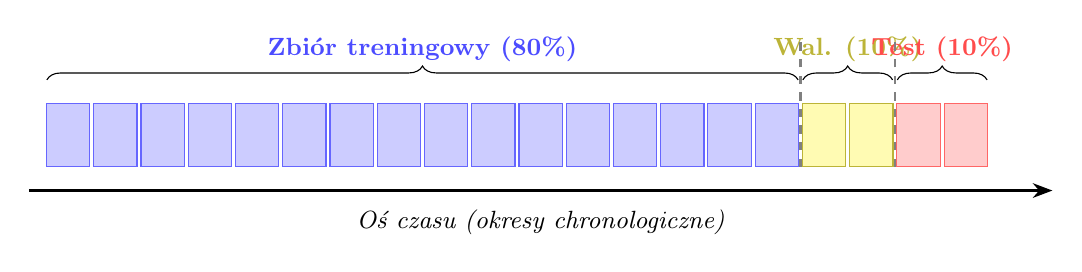
\begin{tikzpicture}[
    train/.style={rectangle, draw=blue!60, fill=blue!20, minimum height=0.8cm, font=\scriptsize},
    val/.style={rectangle, draw=yellow!70!black, fill=yellow!30, minimum height=0.8cm, font=\scriptsize},
    test/.style={rectangle, draw=red!60, fill=red!20, minimum height=0.8cm, font=\scriptsize},
    brace/.style={decorate, decoration={brace, amplitude=5pt, raise=3pt}}
]
    % Train blocks (80%)
    \foreach \i in {0,...,15} {
        \node[train, minimum width=0.55cm] (t\i) at (\i*0.6, 0) {};
    }

    % Val blocks (10%)
    \foreach \i in {16,17} {
        \node[val, minimum width=0.55cm] (t\i) at (\i*0.6, 0) {};
    }

    % Test blocks (10%)
    \foreach \i in {18,19} {
        \node[test, minimum width=0.55cm] (t\i) at (\i*0.6, 0) {};
    }

    % Braces
    \draw[brace] (0*0.6-0.27, 0.6) -- node[above=6pt, font=\small\bfseries, blue!70] {Zbi\'or treningowy (80\%)} (15*0.6+0.27, 0.6);
    \draw[brace] (16*0.6-0.27, 0.6) -- node[above=6pt, font=\small\bfseries, yellow!70!black] {Wal. (10\%)} (17*0.6+0.27, 0.6);
    \draw[brace] (18*0.6-0.27, 0.6) -- node[above=6pt, font=\small\bfseries, red!70] {Test (10\%)} (19*0.6+0.27, 0.6);

    % Time axis
    \draw[-{Stealth[length=2.5mm]}, thick] (-0.5, -0.7) -- (12.5, -0.7);
    \node[font=\small\itshape] at (6, -1.1) {Oś czasu (okresy chronologiczne)};

    % Barrier lines
    \draw[dashed, thick, gray] (15*0.6+0.3, -0.4) -- (15*0.6+0.3, 1.2);
    \draw[dashed, thick, gray] (17*0.6+0.3, -0.4) -- (17*0.6+0.3, 1.2);
\end{tikzpicture}
\caption{Chronologiczny podział danych na zbiory treningowy, walidacyjny i testowy. Przerywane linie oznaczają granice -- dane z późniejszych okresów nigdy nie są używane do trenowania.}
\label{fig:chronological-split}
\end{figure}

Przed podziałem walidowana jest integralność temporalna: weryfikowane jest, czy żadne okresy nie nakładają się między podzbiorami. W przypadku braku informacji o okresach w zbiorze danych, framework automatycznie przechodzi na losowy podział ze stratyfikacją klas.

\subsubsection{Proces trenowania}
\label{subsubsec:trenowanie}

Proces trenowania modeli jest realizowany z wykorzystaniem następujących komponentów:

\begin{itemize}
    \item \textbf{Funkcja straty}: entropia krzyżowa (ang.~\emph{Cross-Entropy Loss}) dla klasyfikacji binarnej:
    \begin{equation}
    \label{eq:cross-entropy}
    \mathcal{L} = -\frac{1}{N}\sum_{i=1}^{N}\left[y_i \log(\hat{y}_i) + (1 - y_i) \log(1 - \hat{y}_i)\right]
    \end{equation}

    \item \textbf{Optymalizator}: Adam z parametrami $\beta_1 = 0{,}9$, $\beta_2 = 0{,}999$.

    \item \textbf{Format danych}: tensory o wymiarach $(\text{seq\_length}, \text{batch\_size}, \text{features}) = (T, B, 100)$, gdzie $T$ jest długością okna (domyślnie 10), $B$ -- rozmiarem wsadu, a 100 -- wymiarem wektora ProtVec.
\end{itemize}

W każdej epoce trenowania stan ukryty LSTM jest odcinany od historii gradientów (ang.~\emph{detach}) na granicach wsadów, co zapobiega propagacji gradientów między niezależnymi próbkami. Selekcja najlepszego modelu odbywa się na podstawie wartości współczynnika MCC (ang.~\emph{Matthews Correlation Coefficient}) na zbiorze walidacyjnym -- zapisywany jest model osiągający najwyższą wartość MCC podczas całego procesu trenowania.

Dla każdego modelu rejestrowana jest pełna historia metryk treningowych i walidacyjnych (strata, dokładność, precyzja, czułość, F1-score, MCC), co umożliwia późniejszą analizę przebiegu trenowania.

\subsubsection{Metryki ewaluacji}
\label{subsubsec:metryki}

Do oceny jakości modeli zastosowano następujący zestaw metryk:

\begin{itemize}
    \item \textbf{Dokładność} (ang.~\emph{Accuracy}) -- udział poprawnie sklasyfikowanych próbek.
    \item \textbf{Precyzja} (ang.~\emph{Precision}) -- udział faktycznych mutacji wśród próbek przewidzianych jako mutacje.
    \item \textbf{Czułość} (ang.~\emph{Recall}) -- udział wykrytych mutacji wśród wszystkich faktycznych mutacji.
    \item \textbf{F1-Score} -- średnia harmoniczna precyzji i czułości.
    \item \textbf{ROC-AUC} -- pole pod krzywą ROC.
\end{itemize}

Główną metryką selekcji modelu jest \textbf{współczynnik korelacji Matthewsa} (ang.~\emph{Matthews Correlation Coefficient}, MCC)~\cite{matthews1975mcc}:

\begin{equation}
\label{eq:mcc-impl}
\text{MCC} = \frac{\text{TP} \cdot \text{TN} - \text{FP} \cdot \text{FN}}{\sqrt{(\text{TP} + \text{FP})(\text{TP} + \text{FN})(\text{TN} + \text{FP})(\text{TN} + \text{FN})}}
\end{equation}

\noindent gdzie TP, TN, FP, FN oznaczają odpowiednio liczby prawdziwie pozytywnych, prawdziwie negatywnych, fałszywie pozytywnych i fałszywie negatywnych klasyfikacji.

MCC przyjmuje wartości z przedziału $[-1, 1]$, gdzie $0$ odpowiada klasyfikatorowi losowemu, $1$ -- idealnej klasyfikacji, a $-1$ -- całkowicie odwrotnej predykcji. Wybór MCC jako głównej metryki jest uzasadniony jego odpornością na niezbalansowanie klas~\cite{chicco2020mcc} -- w odróżnieniu od dokładności, która może być myląca w przypadku skośnego rozkładu klas, MCC uwzględnia wszystkie cztery elementy macierzy pomyłek.

Jako linię bazową (ang.~\emph{baseline}) zastosowano regresję logistyczną (ang.~\emph{Logistic Regression}) na spłaszczonych cechach -- cechy temporalne z $T$ kroków czasowych są konkatenowane w jeden wektor o długości $T \times 100$, który jest podawany na wejście klasyfikatora liniowego. Pozwala to ocenić, czy modele rekurencyjne rzeczywiście wyciągają przydatne informacje z temporalnej struktury danych.

% ============================================================================
\subsection{Aspekty inżynierskie}
\label{subsec:aspekty-inzynierskie}

Oprócz aspektów algorytmicznych, w ramach pracy zaimplementowano szereg rozwiązań inżynierskich mających na celu zapewnienie wydajności, odporności na błędy i reprodukowalności wyników.

\subsubsection{Optymalizacja pamięci i wydajności}
\label{subsubsec:optymalizacja}

Przetwarzanie dużych zbiorów danych sekwencyjnych (rzędu setek tysięcy sekwencji) wymaga świadomego zarządzania zasobami obliczeniowymi:

\begin{itemize}
    \item \textbf{Przetwarzanie wsadowe} -- klasa \texttt{BatchVectorProcessor} realizuje transformację ProtVec w konfigurowalnych wsadach, wykorzystując słownik trigramów z pamięcią podręczną LRU (ang.~\emph{Least Recently Used}) oraz prealokowane tablice NumPy, co eliminuje powtórną alokację pamięci.

    \item \textbf{Mini-Batch K-means} -- dla okresów z dużą liczbą próbek ($> 2000$) automatycznie stosowany jest wariant Mini-Batch~\cite{sculley2010minibatch}, który redukuje złożoność obliczeniową kosztem niewielkiej utraty precyzji klasteryzacji.

    \item \textbf{Strumieniowa deduplikacja} -- dla zbiorów przekraczających 100 tysięcy wierszy deduplikacja jest realizowana w trybie strumieniowym, przetwarzając dane w fragmentach i zapisując wyniki inkrementalnie.

    \item \textbf{Przetwarzanie równoległe} -- etap sortowania sekwencji do okresów czasowych wykorzystuje moduł \texttt{multiprocessing}, a klasteryzacja -- bibliotekę \texttt{joblib} do równoległego przetwarzania plików okresów.
\end{itemize}

\subsubsection{Obsługa błędów i odporność}
\label{subsubsec:obsluga-bledow}

Framework implementuje wielopoziomowy system obsługi błędów:

\begin{itemize}
    \item \textbf{Automatyczne mechanizmy zastępcze} (ang.~\emph{fallbacks}) -- gdy przetwarzanie równoległe nie powiedzie się, framework automatycznie przechodzi na przetwarzanie sekwencyjne. Analogicznie, gdy przetwarzanie strumieniowe zawiedzie, stosowana jest metoda standardowa.

    \item \textbf{Łańcuch kodowań zastępczych} -- przy konwersji plików FASTA testowane są kolejno kodowania: UTF-8, Latin-1, CP1252 i ISO-8859-1.

    \item \textbf{Walidacja spójności konfiguracji} -- przed uruchomieniem każdego etapu sprawdzane jest istnienie wymaganych plików wejściowych i poprawność struktury konfiguracji.

    \item \textbf{Punkty kontrolne} (ang.~\emph{checkpoints}) -- potok przygotowania danych zapisuje postęp po każdym kroku, umożliwiając wznowienie przetwarzania od miejsca przerwania.

    \item \textbf{Logowanie postępu} -- każdy etap raportuje szczegółowe statystyki przetwarzania, w tym liczbę przetworzonych i odrzuconych próbek, czas wykonania oraz zużycie pamięci.
\end{itemize}

\subsubsection{Docker i reprodukowalność}
\label{subsubsec:docker}

W celu zapewnienia reprodukowalności wyników zastosowano następujące mechanizmy:

\begin{itemize}
    \item \textbf{Konteneryzacja Docker} -- środowisko uruchomieniowe jest zdefiniowane w dwuwarstwowej strukturze obrazów:
    \begin{enumerate}
        \item Obraz bazowy (\texttt{base.Dockerfile}) -- oparty na Ubuntu 20.04, zawiera interpreter Python oraz wszystkie zależności (PyTorch, scikit-learn i inne).
        \item Obraz aplikacji (\texttt{Dockerfile}) -- kopiuje kod źródłowy do obrazu bazowego.
    \end{enumerate}
    Taka struktura przyspiesza cykl budowania -- zmiana kodu nie wymaga ponownej instalacji zależności.

    \item \textbf{Stałe ziarno losowości} -- wszystkie operacje stochastyczne używają ustalonego ziarna: \texttt{random\_state=42} dla algorytmów scikit-learn oraz \texttt{torch.manual\_seed(42)} dla operacji PyTorch.

    \item \textbf{Konfiguracja w plikach YAML} -- wszystkie hiperparametry, ścieżki do danych i parametry potoku są zdefiniowane w zewnętrznych plikach konfiguracyjnych, co eliminuje wartości zakodowane na stałe (ang.~\emph{hardcoded}) w kodzie źródłowym i umożliwia pełne odtworzenie eksperymentu.
\end{itemize}

\newpage % Rozdziały zaczynamy od nowej strony.
\section{Wyniki ewaluacji eksperymentalnej}

Niniejszy rozdział przedstawia wyniki eksperymentalnej ewaluacji zaproponowanego frameworku do predykcji mutacji aminokwasowych w białkach wirusowych. Celem przeprowadzonych eksperymentów było zbadanie skuteczności trzech architektur modeli opartych na sieciach LSTM w~zadaniu klasyfikacji binarnej pozycji aminokwasowych jako ulegających bądź nieulegających mutacji. Ewaluację przeprowadzono na dwóch zbiorach danych --- sekwencjach białka S wirusa SARS-CoV-2 oraz białka hemagglutyniny (HA) wirusa Influenza A podtypu H1N1 --- co pozwoliło zweryfikować zdolność frameworku do generalizacji między różnymi patogenami wirusowymi.

%--------------------------------------
\subsection{Środowisko eksperymentalne}
%--------------------------------------

Wszystkie eksperymenty przeprowadzono w~zunifikowanym środowisku obliczeniowym w~celu zapewnienia powtarzalności wyników. Konfiguracja sprzętowa i~programowa została zestawiona w~tabeli~\ref{tab:env}.

\begin{table}[H]
    \centering
    \caption{Konfiguracja środowiska eksperymentalnego.}
    \label{tab:env}
    \begin{tabular}{ll}
        \toprule
        \textbf{Parametr} & \textbf{Wartość} \\
        \midrule
        Procesor graficzny     & % TODO: np. NVIDIA RTX 3090 / Apple M1 Pro \\
        Pamięć RAM             & % TODO: np. 32 GB \\
        System operacyjny      & Ubuntu 20.04 (Docker) \\
        Język programowania    & Python 3.x \\
        Framework ML           & PyTorch~\cite{paszke2019pytorch} \\
        Biblioteka ML          & scikit-learn~\cite{pedregosa2011sklearn} \\
        Ziarno losowości       & 42 \\
        Format konfiguracji    & YAML \\
        \bottomrule
    \end{tabular}
\end{table}

W~celu zapewnienia reprodukowalności wyników zastosowano stałe ziarno losowości (\textit{random seed}) o~wartości 42, które inicjalizowało generatory liczb pseudolosowych w~bibliotekach PyTorch, NumPy oraz wbudowanym module \texttt{random} języka Python. Konfiguracja każdego eksperymentu została zapisana w~pliku YAML, co umożliwia dokładne odtworzenie warunków eksperymentalnych.

%--------------------------------------
\subsection{Zbiory danych}
%--------------------------------------

Ewaluację przeprowadzono na dwóch zbiorach danych, różniących się źródłem, rozmiarem oraz granularnością podziału czasowego. Szczegółowe porównanie parametrów obu zbiorów przedstawiono w~tabeli~\ref{tab:datasets}.

\begin{table}[H]
    \centering
    \caption{Porównanie zbiorów danych wykorzystanych w~eksperymentach.}
    \label{tab:datasets}
    \begin{tabular}{lcc}
        \toprule
        \textbf{Parametr} & \textbf{SARS-CoV-2 Spike} & \textbf{Influenza A H1N1 HA} \\
        \midrule
        Źródło danych          & GISAID~\cite{elbe2017gisaid}  & NCBI~\cite{bao2008ncbi} \\
        Białko                 & Spike (S)                     & Hemagglutynina (HA) \\
        Długość sekwencji      & 1273 aa                       & 565 aa \\
        Liczba epitopów        & 16 regionów (317 poz.)        & 5 miejsc (95 poz.) \\
        Granularność czasowa   & Miesięczna                    & Roczna \\
        Rozmiar zbioru         & $\sim$12\,680 próbek          & $\sim$40\,000 próbek \\
        Okno czasowe           & 10 miesięcy                   & 10 lat \\
        Stosunek mutacji       & $\sim$20\%                    & $\sim$20\% \\
        Podział train/val/test & 80\%\,/\,10\%\,/\,10\%       & 80\%\,/\,10\%\,/\,10\% \\
        \bottomrule
    \end{tabular}
\end{table}

Oba zbiory danych zostały przygotowane z~wykorzystaniem tego samego potoku przetwarzania, obejmującego: filtrowanie sekwencji, kodowanie metodą ProtVec~\cite{asgari2015protvec}, klasteryzację algorytmem K-means~\cite{macqueen1967kmeans} w~ramach poszczególnych okresów czasowych, łączenie klastrów między kolejnymi okresami na podstawie odległości centroidów oraz generowanie próbek treningowych przy użyciu okna przesuwnego. Podział na zbiór treningowy, walidacyjny i~testowy został przeprowadzony chronologicznie --- zbiór testowy obejmuje najnowsze okresy czasowe, co odzwierciedla rzeczywisty scenariusz predykcji przyszłych mutacji.

%--------------------------------------
\subsection{Metryki ewaluacji}
%--------------------------------------

Ze względu na niezbalansowany charakter zadania klasyfikacji binarnej (stosunek klas mutacja/brak mutacji wynosi około 20\%/80\%) zastosowano zestaw metryk uwzględniających tę asymetrię. Oprócz standardowej dokładności (ang.~\textit{accuracy}) wykorzystano następujące miary:

\begin{itemize}
    \item \textbf{Precyzja} (ang.~\textit{precision}) --- stosunek prawidłowo przewidzianych mutacji do~wszystkich przewidzianych mutacji:
    \begin{equation}
        \text{Precision} = \frac{TP}{TP + FP}
        \label{eq:precision}
    \end{equation}

    \item \textbf{Czułość} (ang.~\textit{recall}) --- stosunek prawidłowo przewidzianych mutacji do~wszystkich rzeczywistych mutacji:
    \begin{equation}
        \text{Recall} = \frac{TP}{TP + FN}
        \label{eq:recall}
    \end{equation}

    \item \textbf{Miara F1} (ang.~\textit{F1 score}) --- średnia harmoniczna precyzji i~czułości:
    \begin{equation}
        F_1 = 2 \cdot \frac{\text{Precision} \cdot \text{Recall}}{\text{Precision} + \text{Recall}}
        \label{eq:f1}
    \end{equation}

    \item \textbf{Współczynnik korelacji Matthewsa} (ang.~\textit{Matthews Correlation Coefficient}, MCC)~\cite{matthews1975mcc} --- miara jakości klasyfikacji binarnej uwzględniająca wszystkie elementy macierzy pomyłek:
    \begin{equation}
        \text{MCC} = \frac{TP \cdot TN - FP \cdot FN}{\sqrt{(TP+FP)(TP+FN)(TN+FP)(TN+FN)}}
        \label{eq:mcc-eval}
    \end{equation}

    \item \textbf{Pole pod krzywą ROC} (ang.~\textit{ROC-AUC}) --- miara zdolności modelu do~rozróżniania klas niezależnie od~progu decyzyjnego.
\end{itemize}

Współczynnik MCC przyjmuje wartości z~przedziału $[-1, 1]$, gdzie $1$ oznacza idealną klasyfikację, $0$ --- klasyfikację na poziomie losowym, a~$-1$ --- klasyfikację całkowicie odwrotną. Jak wykazali Chicco i~Jurman~\cite{chicco2020mcc}, MCC stanowi bardziej wiarygodną miarę jakości klasyfikacji binarnej niż dokładność czy miara F1 w~przypadku zbiorów niezbalansowanych, dlatego metryka ta została przyjęta jako główne kryterium porównawcze modeli.

%--------------------------------------
\subsection{Model bazowy}
%--------------------------------------

Jako punkt odniesienia (ang.~\textit{baseline}) dla modeli opartych na sieciach LSTM zastosowano klasyfikator regresji logistycznej (ang.~\textit{Logistic Regression}), zaimplementowany z~wykorzystaniem biblioteki scikit-learn~\cite{pedregosa2011sklearn}. Model bazowy otrzymywał na wejściu spłaszczoną reprezentację okna czasowego --- konkatenację wektorów ProtVec ze~wszystkich kroków czasowych w~oknie --- i~dokonywał klasyfikacji binarnej każdej pozycji aminokwasowej niezależnie. Wybór regresji logistycznej jako modelu bazowego pozwala ocenić, w~jakim stopniu architektury rekurencyjne wykorzystują informację o~zależnościach temporalnych w~porównaniu z~modelem liniowym nieuwzględniającym struktury sekwencyjnej danych.

%--------------------------------------
\subsection{Wyniki dla SARS-CoV-2 Spike}
\label{sec:results-sarscov2}
%--------------------------------------

\subsubsection{Porównanie architektur}

W~tabeli~\ref{tab:results-sarscov2} zestawiono wyniki ewaluacji czterech modeli na zbiorze testowym sekwencji białka S wirusa SARS-CoV-2. Wartości metryk zostały obliczone na zbiorze testowym obejmującym chronologicznie najnowsze okresy czasowe.

\begin{table}[H]
    \centering
    \caption{Porównanie wyników modeli na zbiorze testowym SARS-CoV-2 Spike. Najlepsze wartości dla każdej metryki zostały wyróżnione pogrubieniem.}
    \label{tab:results-sarscov2}
    \begin{tabular}{lcccccc}
        \toprule
        \textbf{Model} & \textbf{Accuracy} & \textbf{Precision} & \textbf{Recall} & \textbf{F1} & \textbf{MCC} & \textbf{ROC-AUC} \\
        \midrule
        Regresja logistyczna    & --- & --- & --- & --- & --- & --- \\
        LSTM                    & --- & --- & --- & --- & --- & --- \\
        Attention LSTM          & --- & --- & --- & --- & --- & --- \\
        Dual Attention LSTM     & --- & --- & --- & --- & --- & --- \\
        \bottomrule
    \end{tabular}
    % TODO: Uzupełnić wartości metryk po przeprowadzeniu eksperymentów.
\end{table}

% TODO: Analiza wyników --- który model osiągnął najlepsze wyniki i z jakiego powodu.
% Oczekiwania: modele z mechanizmem atencji powinny osiągać wyższe wartości MCC
% niż standardowy LSTM, ponieważ mogą selektywnie ważyć informację z różnych
% kroków czasowych okna. Dual Attention LSTM, operujący zarówno na wymiarze
% czasowym, jak i wymiarze cech, powinien osiągnąć najwyższe wartości.

% TODO: Rysunek - krzywe ROC dla wszystkich modeli na jednym wykresie
% \begin{figure}[H]
%     \centering
%     % \includegraphics[width=0.7\textwidth]{rysunki/roc_sarscov2.pdf}
%     \caption{Krzywe ROC dla porównywanych modeli na zbiorze testowym SARS-CoV-2 Spike.}
%     \label{fig:roc-sarscov2}
% \end{figure}

% TODO: Rysunek - macierz pomyłek najlepszego modelu
% \begin{figure}[H]
%     \centering
%     % \includegraphics[width=0.5\textwidth]{rysunki/confusion_matrix_sarscov2.pdf}
%     \caption{Macierz pomyłek najlepszego modelu na zbiorze testowym SARS-CoV-2 Spike.}
%     \label{fig:cm-sarscov2}
% \end{figure}

\subsubsection{Analiza mechanizmu atencji}

Istotną zaletą modeli wyposażonych w~mechanizm atencji jest możliwość interpretacji nauczonych wag, które wskazują, którym krokom czasowym w~oknie przesuwnym model przypisuje największe znaczenie predykcyjne.

% TODO: Rysunek - wizualizacja wag atencji (heatmapa lub wykres słupkowy)
% pokazujący średnie wagi atencji dla poszczególnych kroków czasowych w oknie.
% \begin{figure}[H]
%     \centering
%     % \includegraphics[width=0.7\textwidth]{rysunki/attention_weights_sarscov2.pdf}
%     \caption{Średnie wagi atencji modelu Attention LSTM dla poszczególnych kroków
%              czasowych w oknie przesuwnym (SARS-CoV-2 Spike).}
%     \label{fig:attention-sarscov2}
% \end{figure}

% TODO: Interpretacja biologiczna wag atencji:
% - Czy model przypisuje większą wagę nowszym okresom (bliższym predykowanemu)?
% - Czy obserwuje się wzrost wag w okresach pojawienia się wariantów Alpha, Delta, Omicron?
% - Jakie wnioski biologiczne można wyciągnąć z rozkładu wag atencji?

%--------------------------------------
\subsection{Wyniki dla Influenza A H1N1 HA}
\label{sec:results-influenza}
%--------------------------------------

\subsubsection{Porównanie architektur}

Analogiczną ewaluację przeprowadzono na zbiorze danych sekwencji białka HA wirusa Influenza A podtypu H1N1. Wyniki zestawiono w~tabeli~\ref{tab:results-influenza}.

\begin{table}[H]
    \centering
    \caption{Porównanie wyników modeli na zbiorze testowym Influenza A H1N1 HA. Najlepsze wartości dla każdej metryki zostały wyróżnione pogrubieniem.}
    \label{tab:results-influenza}
    \begin{tabular}{lcccccc}
        \toprule
        \textbf{Model} & \textbf{Accuracy} & \textbf{Precision} & \textbf{Recall} & \textbf{F1} & \textbf{MCC} & \textbf{ROC-AUC} \\
        \midrule
        Regresja logistyczna    & --- & --- & --- & --- & --- & --- \\
        LSTM                    & --- & --- & --- & --- & --- & --- \\
        Attention LSTM          & --- & --- & --- & --- & --- & --- \\
        Dual Attention LSTM     & --- & --- & --- & --- & --- & --- \\
        \bottomrule
    \end{tabular}
    % TODO: Uzupełnić wartości metryk po przeprowadzeniu eksperymentów.
\end{table}

% TODO: Analiza wyników dla Influenza --- porównanie modeli, interpretacja.
% Dane Influenza mają roczną granularność i dłuższą historię ewolucyjną,
% co może wpływać na jakość predykcji w porównaniu z danymi SARS-CoV-2.

\subsubsection{Analiza mechanizmu atencji}

% TODO: Wizualizacja i interpretacja wag atencji dla danych Influenza.
% - Czy rozkład wag różni się od SARS-CoV-2?
% - Jak roczna granularność wpływa na rozkład wag?
% - Czy model identyfikuje lata o szczególnym znaczeniu epidemiologicznym?

% \begin{figure}[H]
%     \centering
%     % \includegraphics[width=0.7\textwidth]{rysunki/attention_weights_influenza.pdf}
%     \caption{Średnie wagi atencji modelu Attention LSTM dla poszczególnych kroków
%              czasowych w oknie przesuwnym (Influenza A H1N1 HA).}
%     \label{fig:attention-influenza}
% \end{figure}

%--------------------------------------
\subsection{Analiza porównawcza}
\label{sec:cross-analysis}
%--------------------------------------

W~celu oceny zdolności frameworku do generalizacji między różnymi białkami wirusowymi przeprowadzono analizę porównawczą wyników uzyskanych dla obu zbiorów danych.

% TODO: Tabela podsumowująca - najlepsze wyniki MCC dla każdego modelu i zbioru danych.
% \begin{table}[H]
%     \centering
%     \caption{Porównanie najlepszych wartości MCC między zbiorami danych.}
%     \label{tab:cross-comparison}
%     \begin{tabular}{lcc}
%         \toprule
%         \textbf{Model} & \textbf{SARS-CoV-2 Spike} & \textbf{Influenza A H1N1 HA} \\
%         \midrule
%         Regresja logistyczna    & --- & --- \\
%         LSTM                    & --- & --- \\
%         Attention LSTM          & --- & --- \\
%         Dual Attention LSTM     & --- & --- \\
%         \bottomrule
%     \end{tabular}
% \end{table}

% TODO: Analiza porównawcza obejmująca następujące aspekty:
% 1. Czy ranking modeli jest spójny między oboma zbiorami danych?
%    Jeśli tak, potwierdza to, że przewaga architektur z atencją jest niezależna
%    od konkretnego białka wirusowego.
% 2. Wpływ rozmiaru zbioru danych na jakość predykcji --- zbiór Influenza
%    jest ponad trzykrotnie większy niż zbiór SARS-CoV-2.
% 3. Wpływ granularności czasowej --- miesięczna (SARS-CoV-2) vs. roczna (Influenza).
% 4. Różnice w dynamice ewolucyjnej obu wirusów i ich przełożenie na wyniki.

%--------------------------------------
\subsection{Dyskusja}
\label{sec:discussion}
%--------------------------------------

% TODO: Interpretacja wyników w kontekście literatury.
% Porównanie z podejściami opartymi na modelach językowych (Hie i in.~\cite{hie2021viral}),
% które wykorzystywały wstępnie wytrenowane reprezentacje sekwencji białkowych
% do przewidywania ucieczki immunologicznej wirusów. W odróżnieniu od tego podejścia,
% zaproponowany framework jawnie modeluje dynamikę temporalną ewolucji wirusowej
% z wykorzystaniem okna przesuwnego i architektur rekurencyjnych.

% TODO: Porównanie z podejściem Mahera i in.~\cite{maher2022predicting},
% którzy zastosowali modele gradient boosting do identyfikacji sterowników
% mutacyjnych wariantów SARS-CoV-2. Zaproponowany framework różni się
% wykorzystaniem informacji temporalnej z wielu kolejnych okresów czasowych
% oraz możliwością zastosowania do różnych białek wirusowych.

% TODO: Omówienie ograniczeń eksperymentów:
% - Zależność od jakości danych źródłowych (bias w próbkowaniu sekwencji).
% - Wpływ progów klasteryzacji na jakość predykcji.
% - Ograniczenia wynikające z binarnej natury predykcji (mutacja/brak mutacji)
%   w porównaniu z predykcją konkretnego aminokwasu substytucyjnego.
% - Brak walidacji prospektywnej na danych z przyszłych okresów.

% TODO: Wnioski z eksperymentów:
% - Podsumowanie, która architektura okazała się najskuteczniejsza.
% - Ocena, czy mechanizm atencji wnosi istotną poprawę.
% - Ocena konfigurowalności i reprodukowalności frameworku.
% - Wnioski dotyczące generalizowalności między różnymi białkami wirusowymi.

\newpage
\section{Podsumowanie}

W~ramach niniejszej pracy zaprojektowano i~zaimplementowano konfigurowalny framework do predykcji mutacji aminokwasowych w~białkach wirusowych z~wykorzystaniem rekurencyjnych sieci neuronowych. Opracowany system przetwarza surowe pliki FASTA poprzez pięcioetapowy potok obejmujący: czyszczenie i~filtrowanie sekwencji, podział na okresy czasowe, klasteryzację K-means z~wykorzystaniem reprezentacji ProtVec, dwukierunkowe łączenie klastrów między kolejnymi okresami oraz tworzenie zbiorów danych z~oknem przesuwnym z~ekstrakcją regionów epitopowych. Zaimplementowano trzy architektury modeli o~rosnącej złożoności --- bazowy model LSTM, model LSTM z~mechanizmem atencji Bahdanau oraz model LSTM z~podwójną atencją (DA-RNN) --- co umożliwiło systematyczne zbadanie wpływu mechanizmów atencji na jakość predykcji. Całość rozwiązania skonteneryzowano z~wykorzystaniem platformy Docker, a~konfigurację poszczególnych eksperymentów zrealizowano za pomocą plików YAML, co zapewnia reprodukowalność wyników oraz łatwość adaptacji frameworka do nowych patogenów.

% TODO: Uzupełnić po zakończeniu eksperymentów
Wyniki ewaluacji eksperymentalnej przeprowadzonej na dwóch zbiorach danych --- sekwencjach białka~S wirusa SARS-CoV-2 oraz białka HA wirusa Influenza~A podtypu H1N1 --- pozwoliły na częściową weryfikację postawionej tezy badawczej. Zastosowanie chronologicznego podziału danych, w~którym zbiór testowy obejmował wyłącznie okresy czasowe następujące po danych treningowych, zapewniło realistyczną ocenę zdolności predykcyjnych modeli, eliminując ryzyko wycieku informacji z~przyszłości do zbioru treningowego. [Placeholder: Model z~podwójną atencją osiągnął najwyższe/porównywalne wartości MCC wynoszące \ldots, co potwierdza/nie potwierdza hipotezę, że mechanizmy atencji poprawiają jakość predykcji mutacji w~regionach epitopowych.]

Przeprowadzona analiza pozwala na sformułowanie oceny zarówno zalet, jak i~ograniczeń zaproponowanego podejścia. Do istotnych zalet frameworka należy jego uniwersalność --- wykazano możliwość zastosowania tego samego potoku przetwarzania dla dwóch odrębnych wirusów przy zmianie wyłącznie pliku konfiguracyjnego YAML. Konteneryzacja Docker zapewnia pełną reprodukowalność środowiska obliczeniowego, natomiast modułowa architektura systemu ułatwia wymianę poszczególnych komponentów, na przykład zastąpienie algorytmu klasteryzacji lub modelu predykcyjnego. Wśród ograniczeń należy wskazać przede wszystkim binarny charakter predykcji --- framework przewiduje jedynie, czy w~danym regionie epitopowym nastąpi mutacja, nie precyzując jednak, jaki konkretnie aminokwas zastąpi dotychczasowy. Ponadto jakość uzyskiwanych wyników jest uzależniona od kompletności i~reprezentatywności danych dostępnych w~bazach GISAID oraz NCBI, co w~przypadku nowo pojawiających się patogenów może stanowić istotne ograniczenie. [Placeholder: Dodatkowe ograniczenia wynikające z~wyników eksperymentalnych.]

Na podstawie przeprowadzonych badań sformułowano następujące wnioski. Reprezentacje ProtVec, oparte na analogii między trójkami aminokwasów a~słowami w~przetwarzaniu języka naturalnego, stanowią skuteczny sposób kodowania sekwencji białkowych zarówno na potrzeby klasteryzacji, jak i~modelowania z~użyciem sieci neuronowych. Klasteryzacja K-means zastosowana do reprezentacji ProtVec pozwala na redukcję złożoności danych przy jednoczesnym zachowaniu informacji o~dominujących wzorcach sekwencyjnych w~poszczególnych okresach czasowych. Mechanizmy atencji umożliwiają modelowi selektywne przypisywanie różnych wag poszczególnym krokom czasowym w~oknie wejściowym, co jest szczególnie istotne w~kontekście nierównomiernej dynamiki ewolucji wirusowej. Zaproponowany framework, dzięki swojej konfigurowalności, może zostać rozszerzony na inne białka wirusowe bez konieczności modyfikacji kodu źródłowego.

Wyniki niniejszej pracy otwierają szereg kierunków dalszych badań. Po pierwsze, zasadne byłoby rozszerzenie zestawu architektur modelowych o~modele oparte na mechanizmie samoatencji (ang.~\textit{self-attention}), w~szczególności architektury Transformer, które w~wielu dziedzinach przetwarzania sekwencji wykazują przewagę nad klasycznymi modelami rekurencyjnymi. Po drugie, istotnym rozwinięciem byłoby przejście z~predykcji binarnej na predykcję konkretnych substytucji aminokwasowych, co wymagałoby przeformułowania problemu jako klasyfikacji wieloetykietowej (ang.~\textit{multi-label classification}). Po trzecie, integracja danych dotyczących trójwymiarowej struktury białek, na przykład pochodzących z~modeli AlphaFold, z~informacjami sekwencyjnymi mogłaby wzbogacić reprezentację wejściową i~poprawić jakość predykcji. Po czwarte, framework może zostać rozszerzony o~obsługę kolejnych wirusów --- na przykład HIV czy wirusa Ebola --- oraz innych białek powierzchniowych. Po piąte, systematyczna optymalizacja hiperparametrów z~wykorzystaniem metod takich jak optymalizacja bayesowska (ang.~\textit{Bayesian optimization}) mogłaby doprowadzić do poprawy wyników bez modyfikacji samej architektury modelu. Wreszcie, opracowanie modeli wielozadaniowych (ang.~\textit{multi-task learning}), łączących predykcję mutacji z~klasyfikacją wariantów wirusa, stanowi obiecujący kierunek pozwalający na jednoczesne wykorzystanie komplementarnych sygnałów zawartych w~danych.


\cleardoublepage % Zaczynamy od nieparzystej strony
\printbibliography

% Spisy (opcjonalne)
\newpage
\pagestyle{plain}

\vspace{0.8cm}


\listoffigurestoc
\vspace{1cm}
\listoftablestoc

\end{document}